
%(BEGIN_QUESTION)
% Copyright 2006, Tony R. Kuphaldt, released under the Creative Commons Attribution License (v 1.0)
% This means you may do almost anything with this work of mine, so long as you give me proper credit

Weirs and flumes are frequently equipped with stilling wells to provide a ``quiet'' liquid height for an instrument to measure, usually an ultrasonic or displacer sensor such as the type used to measure liquid level in a closed vessel:

$$\includegraphics[width=15.5cm]{i00624x01.eps}$$

This level-sensing instrument usually provides the characterization necessary to linearize the weir or flume's nonlinear flow/height response.  If the level-sensing instrument is ultrasonic, the flow characterization may be done in the same digital computer that calculates liquid level by timing the sound echoes.  

However, there is a low-technology way to do the same thing.  If we use a displacer rather than a digital ultrasonic sensor, we may perform this same characterization by carefully choosing the correct non-cylindrical displacer shape, so that liquid height in the stilling well does not linearly translate to buoyant force felt by the transmitter unit.

\vskip 10pt

Suppose we are setting up a transmitter on a Cippoletti weir, whose flow rate varies with the 1.5 power of liquid height in the stilling well ($Q \propto H^{1.5}$).  Choose the correct profile of displacer for this application, to properly linearize the liquid height into a flow signal that we may read directly:

$$\includegraphics[width=15.5cm]{i00624x02.eps}$$

\underbar{file i00624}
%(END_QUESTION)





%(BEGIN_ANSWER)

$$
\includegraphics[width=15.5cm]{i00624x03.eps}$$

Now, explain {\it why} the displacer must have this kind of shape, and not one of the other shapes!  Hint: sketch a graph of the weir's flow/height transfer function.

%(END_ANSWER)





%(BEGIN_NOTES)


%INDEX% Measurement, flow: transfer functions of weirs and flumes

%(END_NOTES)


